\begin{abstract}

When a recovery branch succeeds, does it identify an intervention worth repeating? We investigate the gap between observed rescue and repeatable intervention value in vision-language-action policies. Our evaluation combines saved-state branching, same-policy pseudo-options, separate selection and evaluation blocks, and complete deadline readouts. We analyze observation refresh for $\pi_0$ and a structured detour for OpenVLA, then test locked forecasts in 332 new executions of existing states. The results distinguish different kinds of recovery evidence. One-shot Refresh selection at 100 actions gains 12.50 percentage points on the outcomes used to select it, 3.12 points on a separate block, and zero on the prospective block. Its remaining full-repeat positive contribution is explained by local acceleration across the evaluation deadline. In contrast, full-repeat Detour selection at 440 actions retains gains of 6.25, 4.17, and 5.21 points across the three blocks, including two sources with benefit in every block. The same-policy negative control generates apparent gains without a distinct recovery action. Separate-block forecasting improves the one-shot comparisons, but does not uniformly improve source-level prediction for full-repeat references. These scoped results show why observed rescue, repeatable benefit, and deployable selection need distinct evidence: some opportunities disappear, some persist, and a single replication can also miss an opportunity that reappears later.


\end{abstract}

\section{Introduction}

A robot reaches a difficult manipulation state. A recovery routine takes over and completes the task. This is a valuable demonstration: the alternative controller can accomplish something the observed continuation did not. To decide whether a future robot should intervene in that state, however, the relevant quantity is the expected improvement over continuing the original policy. A successful alternative and one unsuccessful continuation do not determine that quantity.


The distinction becomes tangible in a saved-state manipulation example. From the same Detour-study bundle, one Base execution collides and another succeeds. The structured alternative succeeds in both corresponding executions. The first comparison appears to demonstrate rescue; the second demonstrates successful but unnecessary intervention. A complementary example has repeated Base accidents and repeated Detour successes. Both examples belong in an evaluation: the first exposes ambiguity, while the second preserves constructive evidence of recovery.


This paper asks how to distinguish these cases before attributing performance to an intervention selector. We use a simulator to execute fixed alternatives from saved decision states and retain repeated outcomes, source identity, and complete budget readouts. This setting makes a particularly simple negative control possible: label two executions of Base as two pseudo-options and apply the same hindsight selection rule. Any apparent improvement then arises without introducing a different recovery controller. The negative control diagnoses a property of the evaluation; it is not a deployable action and is not a numerical noise correction for real recovery.


Three separations organize the investigation. First, selecting and scoring with the same outcomes measures a different object from evaluating the frozen selection on subsequent executions. Second, finishing just before a deadline can differ from rescuing a task that would otherwise terminate in an accident. Third, an opportunity identified using actual branch outcomes can remain inaccessible to a selector that must act using its current observations. Each distinction changes what a positive result warrants.


Our evidence comes from two policy interfaces and three development panels. The same diagnostic procedure differentiates their results: a Refresh panel has deadline-sensitive and repeat-sensitive selection value, a second Refresh panel has no observed task-selection gain, and Detour retains several actual rescues while damaging many nominally successful tasks when applied indiscriminately.


Our contribution is a prospective empirical study of what recovery evidence predicts. We lock choices and forecasts before 332 new executions, and find opportunities that disappear, opportunities that persist, and one that disappears in a replication and returns in the next. This changes the research decision: deadline-sensitive acceleration calls for an efficiency objective; persistent benefit calls for a selector that can identify it; missing benefit support calls for examining the recovery skill and state population. The evaluation connects observed outcomes to these different next steps. Sample splitting and selection bias are established statistical ideas; the empirical question is whether they change the conclusion about a particular VLA intervention.


\section{Intervention value and its measurement}

Let B denote the nominal policy and R a fixed alternative. For a saved decision state s and a declared action budget h, $Y_a(s,h)$ is one when executing a completes the task before an accident and within h; otherwise it is zero. The expectation $q_a(s,h)$ is defined with respect to the declared continuation and runtime execution mechanism. The relevant success difference is


\begin{equation}\Delta_R(s,h)=q_R(s,h)-q_B(s,h).\end{equation}

The state includes the simulator, controller, policy continuation, delivered observation, and any queued actions. Matching the starting state does not assert that all subsequent inputs or computations are deterministic. Runtime variation therefore remains part of the empirical measurement, even under greedy decoding.


A state where R succeeds can still have zero intervention benefit because Base also succeeds. Conversely, avoiding an accident without completing the task may improve a safety objective while leaving this task-success difference unchanged. We consequently report accident outcomes, lost Base successes, and new accidents alongside success gain. We do not collapse these outcomes into a freely selected utility coefficient.


Two idealized quantities clarify the learning problem. With full state access, the positive intervention opportunity is $\Omega$; with only the execution-time input X, the available opportunity is $\Omega_X$:


\begin{equation}\begin{gathered}\Omega=E_s[\max(0,\Delta_R(s,h))],\\ \Omega_X=E_X[\max(0,E[\Delta_R(s,h)\mid X])],\\ \Omega_X\leq\Omega.\end{gathered}\end{equation}

The standard ordering of these quantities separates benefit support from the ability to recognize it. Our finite-repetition reference estimates neither quantity exactly. Its role is diagnostic: a failed learned selector alone cannot tell us whether the fixed recovery has little value, the available inputs hide that value, or the learner fails to use informative inputs.


For diagnostic choice, let $\delta_A$(s) select R only when its mean success in execution block A exceeds Base's; ties retain Base. We measure the same fixed choice using the A and B outcomes:


\begin{equation}\begin{gathered}G_A=E_s[\delta_A(s)(\bar Y_{R,A}-\bar Y_{B,A})],\\ G_B=E_s[\delta_A(s)(\bar Y_{R,B}-\bar Y_{B,B})].\end{gathered}\end{equation}

$G_A$ reuses the outcomes that determined the choice. $G_B$ evaluates that choice on a separate execution block. Neither is a new-source generalization result; both use the same physical decision states. In particular, $G_B$ is not a certified upper bound on achievable value, since a finite-sample A choice can miss beneficial states.


An important boundary follows. A pre-specified intervention evaluated through an appropriately sampled one-shot paired mean need not be biased. Our concern is reusing the outcome to select its winner, treating a single realization as a deterministic recoverability label, or interpreting a hindsight oracle as the value available to an execution-time learner. No claim requires repeating every training state, and noisy outcomes can still support learning expected values.


Even identical policies can produce positive reused value. For two IID executions with success probability q, selecting the better outcome yields expected apparent gain q(1-q), or 25 points at q=0.5; a fresh independent pair has zero expected gain. Appendix C gives the elementary calculation. Actual runtime blocks need not satisfy these IID assumptions, so we report their observed pseudo-value directly.


\section{Protocol and evidence}

\subsection{Frozen panels}

We use OpenVLA~\citep{kim2024openvla} and pi0~\citep{black2024pi0} policies in LIBERO~\citep{liu2023libero} manipulation tasks.


\begin{center}\small\setlength{\tabcolsep}{3pt}

\begin{tabularx}{\linewidth}{>{\raggedright\arraybackslash}X >{\raggedright\arraybackslash}X >{\raggedright\arraybackslash}X >{\raggedright\arraybackslash}X}

\toprule

\textbf{Panel / policy} & \textbf{Sources / decisions} & \textbf{A/B repeats per arm} & \textbf{Budgets} \\

\midrule

Candidate Refresh / $\pi_0$ & 8 / 18 & 4 / 4 & 100, 200 suffix actions \\

Selection retest / $\pi_0$ & 12 / 24 & 4 / 4 & 100 suffix actions \\

Detour / OpenVLA & 16 / 48 & 2 / 2 & 220, 440 episode actions \\

\bottomrule\end{tabularx}\end{center}

Candidate Refresh comprises all nine historical stale-success configurations and nine matched-buffer controls; it is a selected development panel. The selection retest used a separate fixed training-source panel that did not reproduce those nine configurations. Detour uses on-path glass, off-path glass, and no-glass conditions for each source. One Detour episode terminates before a candidate is available and is preserved as a shared outcome, without fabricating repeated branches.


All panels were exposed during earlier development. The new analysis does not restore their blind-test status. Detour's recovery controller uses privileged geometry and fixed stage targets. Refresh clears a software observation queue and requeries the same $\pi_0$ policy once; it does not permanently eliminate sensor delay. The Refresh panels share source pools; their sources are not added into a larger independent sample. Mechanisms retain their original clocks and accident predicates.


\subsection{Real and pseudo-option selection}

We report two principal real-intervention views. The one-shot view selects from the first A execution of each arm and evaluates the first B execution. The full-repeat view uses all available A repetitions to select and all B repetitions to evaluate. The original historical references, whose objectives can additionally prioritize accident reduction on success ties, are scored separately without change.


For the same-policy negative control, pseudo-arm 0 and pseudo-arm 1 are the first and second Base executions within each block. The A winner's index is fixed before reading its B value. A predeclared swapped orientation exposes sensitivity to the arbitrary indexing. When four repetitions are available, an additional comparison uses two executions per pseudo-arm, paired with a real two-repetition comparison. These alternative assignments are dependent diagnostics and do not increase the number of independent samples.


All aggregate values first average decisions within physical source and then average sources. Treatment, controls, fitting, and calibration are also reported separately. Uncertainty intervals use 5,000 paired physical-source bootstrap draws and describe these development panels. A zero interval for identical recorded contributions is not a population safety guarantee.


\subsection{Budget readouts}

Each available short and long outcome comes from the same continuous trajectory. For every A choice, we keep the choice fixed along the entire success and accident curve. This separates a new execution's effect from a changed deadline's effect. Detour includes its prefix and recovery actions in the episode budget; Refresh uses the original suffix action budget. We preserve this distinction rather than combining their action counts into one measure of recovery speed.


\section{Existing-record results}

\subsection{Outcome reuse has heterogeneous effects}

All gains are physical-source-weighted safe-task-success percentage points, with every condition included. One-shot Refresh at 100 actions changes from 12.50 in A to 3.12 in B; full-repeat selection changes from 7.03 to 5.47. At 200 actions, the full-repeat gain changes from 1.56 to zero. In contrast, Detour at 440 retains 6.25 in A and 4.17 in B. The selection-retest panel has zero observed gain. Appendix A retains every declared budget and its source interval.


These effects are heterogeneous. Increasing repetitions also changes the selected policy, so the Refresh comparison is not a universal sample-size law. Detour's retained gain directly contradicts an interpretation that all observed recovery value disappears on a separate block.


\begin{figure}[tb]\centering

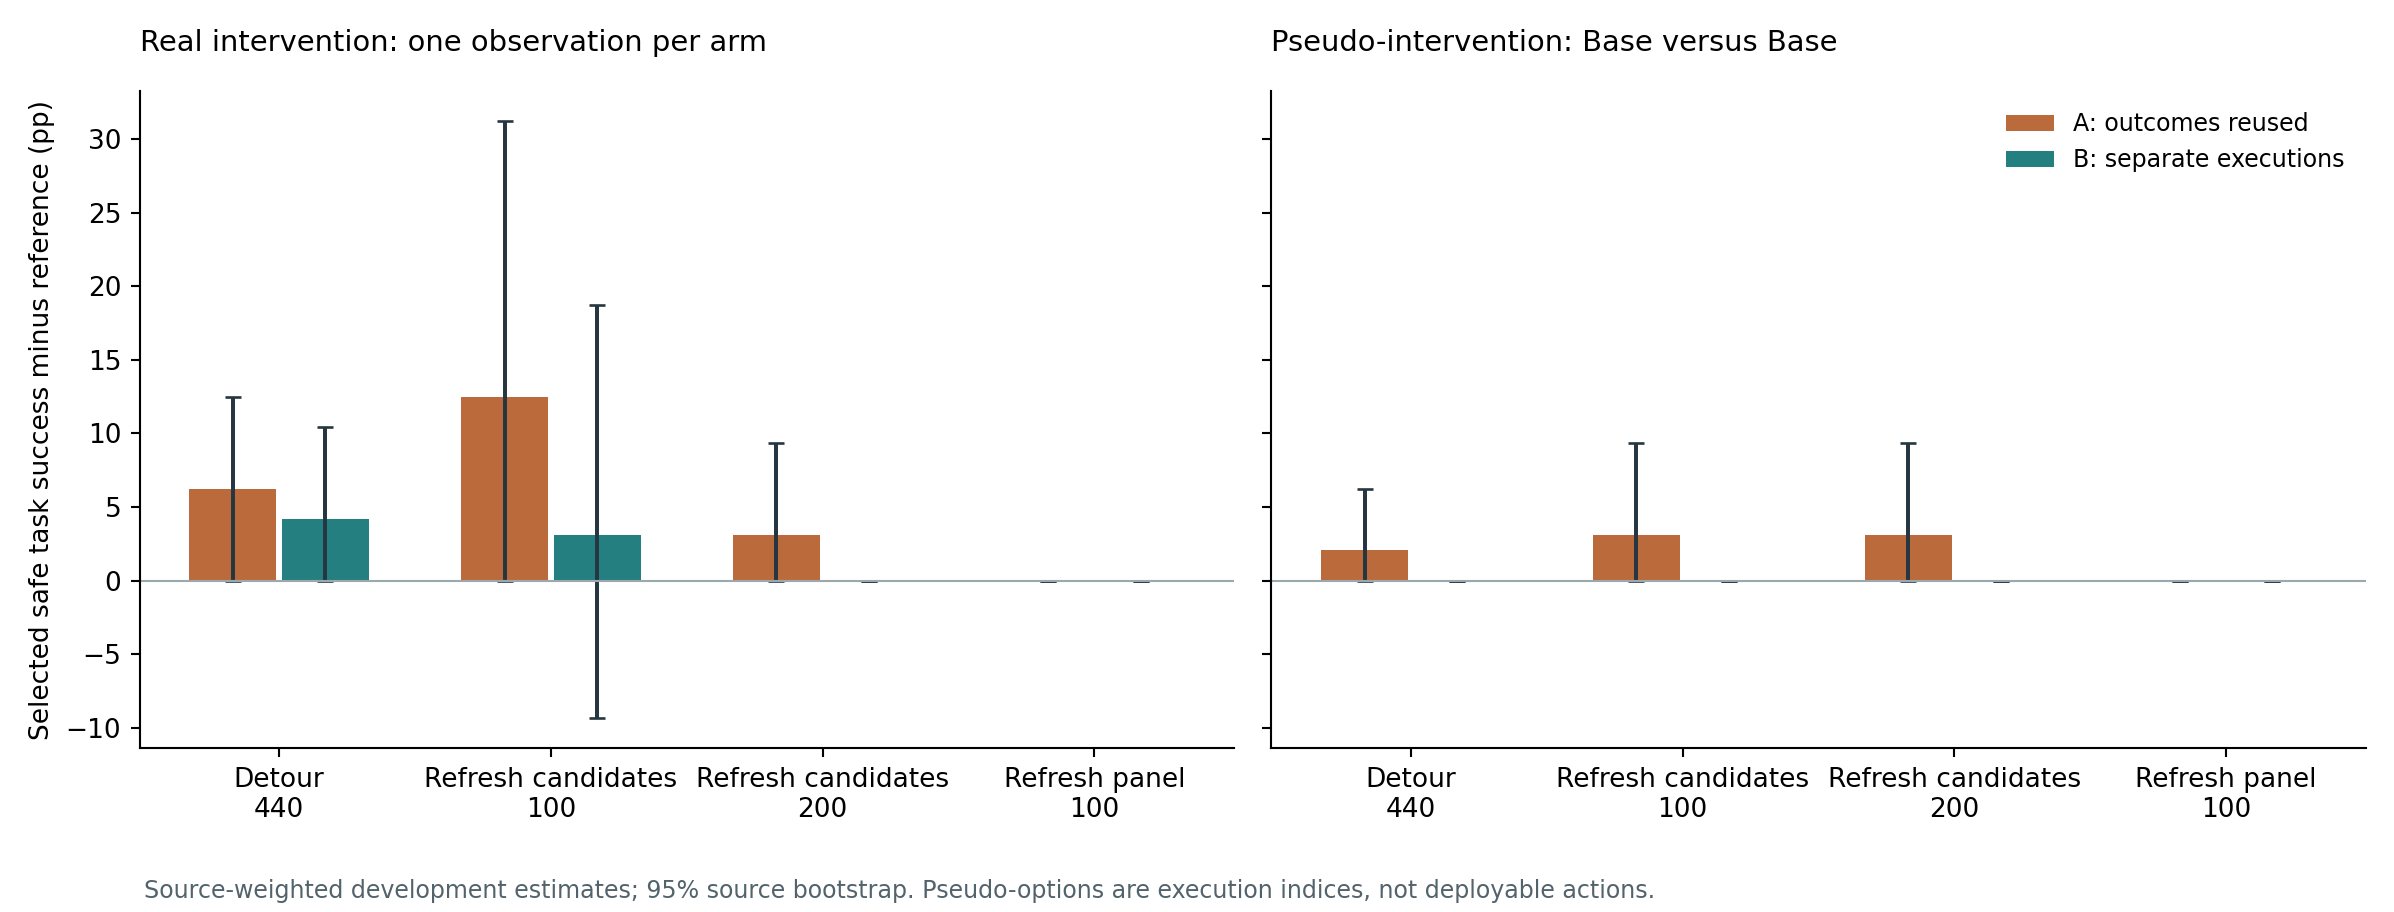
\includegraphics[width=\linewidth]{../../../audits/20260913/repeat_value/evidence/real_and_pseudo.png}

\caption{Matched one-observation-per-arm diagnostics. Left: a real alternative to Base. Right: two execution indices of Base. Bars are source-weighted estimates; intervals are descriptive source bootstraps. The pseudo-options do not exist as distinct deployable actions. Swapped and two-repeat variants are retained in the full evidence, rather than selected after observing favorable contrasts.}

\end{figure}

\subsection{A pseudo-option can appear beneficial}

At 440 actions, the first-orientation Detour Base/Base control shows 2.08 points of apparent gain in A and zero in B. Swapping the pseudo-arm identities produces 6.25 points in A and 2.08 in B. Candidate Refresh at 100 actions shows 3.12 points in A and zero in B under the first one-shot assignment; its swapped assignment is zero in both blocks. The selection-retest panel is zero throughout these success diagnostics.


The orientation dependence is informative. It prevents interpreting the control as a precise estimate of a universal noise floor. In the two-repeat Refresh assignment at 100 actions, pseudo-value even retains 3.12 of its 7.81 apparent points on B. A separate block is an empirical check, not an automatic certificate that a remaining positive value corresponds to a distinct useful action.


\subsection{A deadline can change the meaning of rescue}

In the candidate study's B stale executions, Base and Refresh succeed 23/36 and 26/36 times at 100 actions, but 33/36 and 31/36 times at 200 actions. These are raw execution counts, distinct from the source-weighted selection table above. All five positive paired conversions at 100 have a Base continuation that succeeds at action 101 or 102. The shorter deadline measures a completion-time advantage for these cases; it does not establish rescue from persistent inability to complete. This acceleration is measured in environment actions. A practical latency objective would also need to account for Refresh's additional inference cost.


The selected policy also changes its apparent value under this check. Keeping the same one-shot A choice from the 100-action budget, its B gain changes from +3.12 points at 100 to -3.12 points at 200. The full-repeat 100-action choice has zero net B gain at 200, while still losing some Base successes and introducing a new accident. The longer readout therefore reveals more than disappearance of a binary advantage: it can reveal a cost of an intervention that appeared useful at the shorter deadline.


Detour supplies a complementary pattern. At e18 and e21, A/B contain four Base accidents per state and four Detour completions. Detour completes at episode actions 202 and 432 respectively. The latter requires the longer budget, but its advantage is not explained by a Base continuation succeeding one or two actions later.


\begin{figure}[tb]\centering

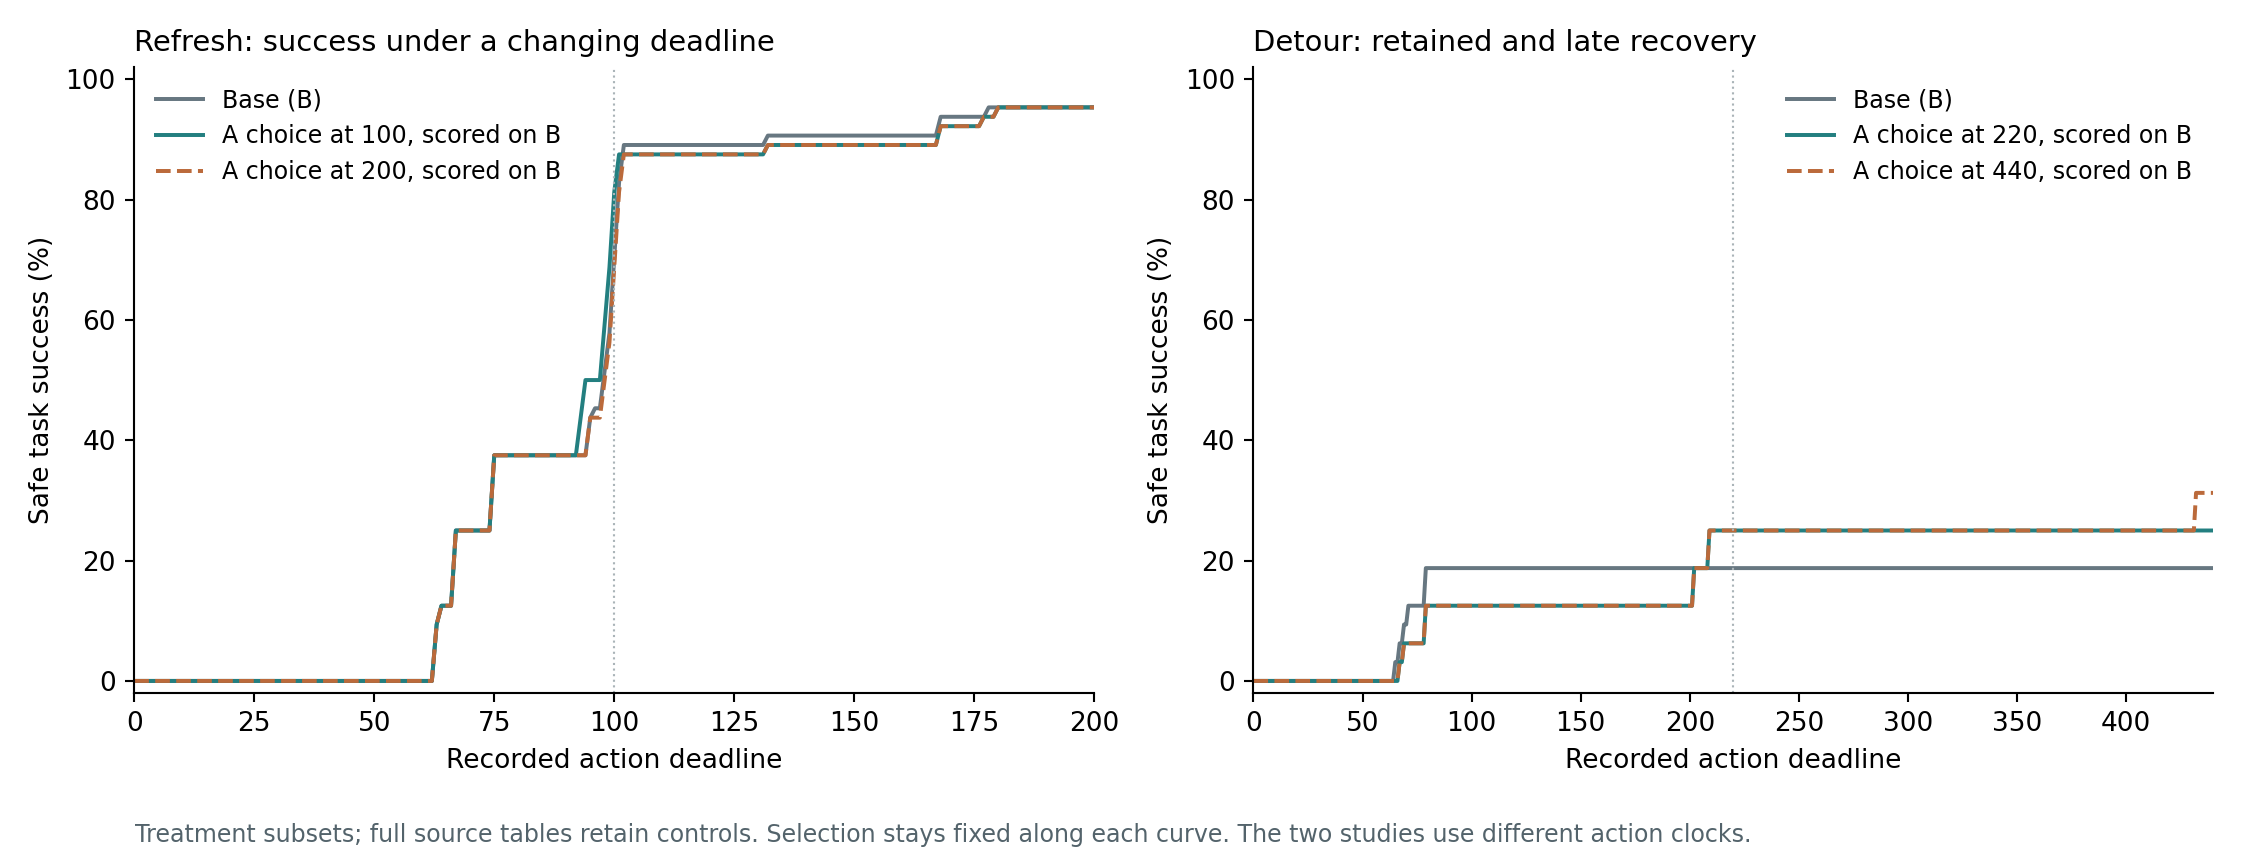
\includegraphics[width=\linewidth]{../../../audits/20260913/repeat_value/evidence/deadline_curves.png}

\caption{Treatment-condition success curves on B for A choices fixed at the original deadlines. Controls remain in aggregate tables. The studies use different action clocks; the curves illustrate different effects of time without selecting a new favorable primary deadline.}

\end{figure}

\subsection{Retained opportunity is not yet deployable value}

Detour's A-to-B positive-success intersection contains e18 and e21, both fitting sources. The calibration sources have no positive B success-difference cell. The full-input gate therefore offers no additional observed task gain: it selects Base throughout and achieves the same 67.71\% success. AlwaysDetour reaches 39.58\% at 440 actions, and the strong risk-to-Detour reference reaches 63.54\%.


The full gate was calibrated for 220-action success, with accident conditions at both budgets. This is a material limitation when interpreting long-budget e21: the experiment did not independently develop a 440-action gate. Nevertheless, changing that target would not by itself establish positive calibration support or protect normal task success. The data currently distinguish actual recovery examples from an effective execution-time selection method.


\section{Prospective execution-block replication}

The existing-record results motivated one bounded new C block. Before any C execution, we recorded all A choices, A/B value forecasts, input hashes, checkpoint identities and scoring rules. The experiment reuses the complete saved states from both primary panels: 188 Detour branches and 144 candidate Refresh branches, with no new prefixes or physical sources. Each panel runs in a process separate from its A/B collection and preserves its original budget and continuation contract.


For each frozen choice, we compare the forecasts $G_A$ and $G_B$ with the new $G_C$. We also compare source-level squared prediction errors. The procedure allows either forecast to win: a positive error-improvement contrast favors B, whereas a negative contrast favors A. C itself has finite repetitions and is not an exact measurement of the expected intervention value. All pseudo-option assignments and historical frozen references remain visible.


\subsection{Refresh: a prospective check changes the value estimate}

The Refresh C block completed all 144 branches. The one-shot 100-action reference progresses from 12.50 points in A to 3.12 in B to 0.00 in C. The full-repeat reference retains 2.34 points at 100 actions, but reaches -0.78 at 200. Choices and forecasts were fixed before this new execution block.


The complete budget-by-reference table is in Appendix A.


The two reference types use their stated number of observations per arm in each block; they differ in both selection and evaluation, not just in the precision of a common C target. Values and RMSE are in percentage points. The full-repeat C gain at 100 has a descriptive source interval [-4.69,13.28], and the 200-action gain has interval [-2.34,0.00].


Forecast accuracy is mixed. B is closer than A to C for the one-shot 100 reference, including source-level prediction error. For the four-repeat 100 reference, B's aggregate value is closer, but its source-level RMSE is higher. The predeclared squared-error improvement contrast is -0.01758 in squared probability units, with descriptive interval [-0.04883,0.01367]. Thus separating a single estimation block does not establish a generally better forecast of source-specific value. The third block is useful because it can expose this failure rather than assume the forecast improved.


The retained 2.34-point full-repeat gain at 100 also includes 3.91 points of lost Base successes and 0.78 points of new accidents. Both must accompany the net result. At 200, the selected policy loses 0.78 points of success and introduces 0.78 points of new accidents. The one-shot pseudo-options score zero in C at both budgets; the full evidence retains two-repeat and swapped-index controls as specified.


The residual short-budget value has a concrete explanation. At 100 actions the full-repeat C reference has one source with a positive net contribution and two with negative contributions. Its positive selected anchor b14 has Base completion times 95, 104, 101, 105 and Refresh completion times 95, 94, 94, 94. All eight branches complete by 105 actions. Thus the positive C contribution preserves local acceleration, while its apparent task-rescue interpretation remains deadline-sensitive.


\begin{figure}[tb]\centering

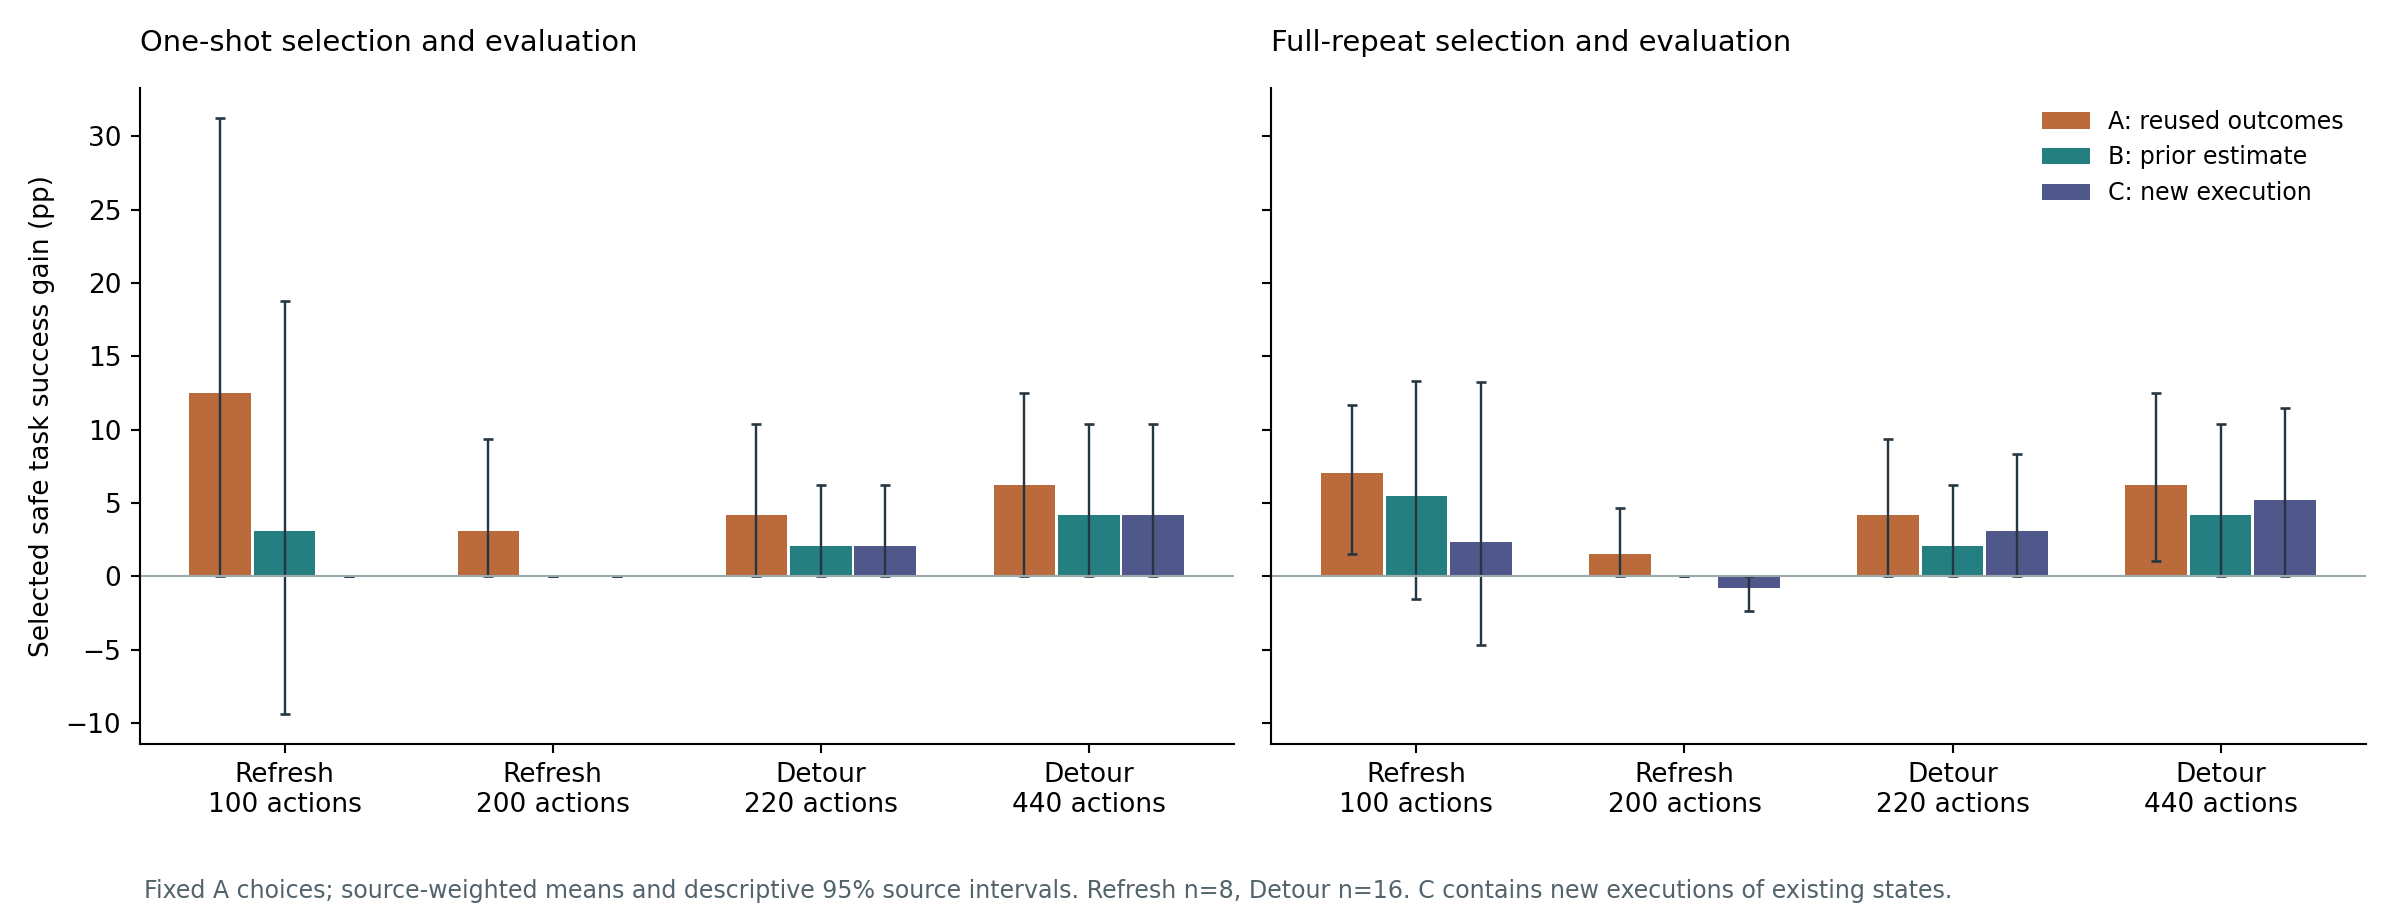
\includegraphics[width=\linewidth]{../../../audits/20260913/repeat_value/paper_figure/abc_value.png}

\caption{A choices and A/B forecasts locked before 332 new executions. Both one-shot and full-repeat references appear at every original budget. Source-weighted means and descriptive source intervals are shown; physical sources remain the same across execution blocks. Pseudo-options and all historical policies are retained in the full accompanying tables.}

\end{figure}

\subsection{Detour: task benefit survives, while one replication can miss it}

The Detour C block completed all 188 branches. Full-repeat selection retains 5.21 points of gain at 440 actions, compared with 6.25 in A and 4.17 in B. The C success rates are 69.79\% for the fixed A reference and 64.58\% for Base; the gain has a descriptive source interval of [0.00, 11.46] points. The selected reference has no observed lost Base success or new accident in C.


Figure 3 retains both budgets and both reference types; Appendix A gives their values.


The constructive cases remain e18 and e21: both have positive benefit in A, B, and C. Detour's C executions finish at 202 and 432 episode actions respectively. The e18 Base outcomes in C are an accident and noncompletion at 440; the e21 Base outcomes are two accidents. These are not the short catch-up pattern observed in Refresh. They establish finite-budget recovery benefit on these saved states.


A third source illustrates the other direction of error. At e15, full-repeat benefit changes from 0.5 in A to zero in B and back to 0.5 in C. The C Base executions succeed at action 70 and collide at action 41, while both Detour executions succeed at 209. Rejecting this opportunity solely because B had zero observed gain would therefore miss its subsequent reappearance. All three positive C sources are on the fitting side; calibration still has no positive success-difference cell. The learned gate remains Base throughout, with C success 64.58\%, compared with 60.42\% for the strong risk reference and 39.58\% for AlwaysDetour.


For full-repeat Detour, A and B have equal source-level forecast RMSE, and the predeclared error-improvement contrast is zero, with interval [-0.00521, 0.00521]. Together with the Refresh result, this limits the strong claim that one separate estimation block generally improves source-specific value prediction. The useful conclusion is empirical: prospective execution distinguishes gains that disappear, gains that persist, and opportunities whose evidence varies across small blocks.


\section{Related work and the contribution boundary}

SAFE~\citep{gu2025safe} develops failure detection using internal VLA features. Our question concerns the consequences of alternative actions after a candidate state is identified; it does not introduce a new hidden-state detector. LIBERO-RECOVER~\citep{liu2026recover} evaluates recovery across a much larger collection of failure scenarios. Our panels do not compete on benchmark breadth, and the contribution cannot be the existence of recovery evaluation alone.


B2FF~\citep{shin2026b2ff} trains a recoverability-aware milestone selector using counterfactual rollout supervision. It includes an online-triggered variant as well as controlled recovery timing and timing ablations. Our diagnostics address the interpretation of realized option outcomes; they do not establish that B2FF's reported results suffer the same effect. CoRe~\citep{zhang2026core} studies inference-time recovery through counterfactual realignment. A direct comparison would need to align recovery permissions, physical costs and accident definitions, rather than compare unmatched success rates.


See, Plan, Rewind~\citep{dai2026spr} learns a brief retraction operation and uses progress anomalies to trigger it. It offers a concrete external mechanism for testing whether our observations extend beyond queue refresh and a structured geometric detour. Availability of an external model is distinct from a completed replication; the present performance tables contain our two evaluated interfaces.


VoLoAgent~\citep{chen2026volo} combines VLA execution with VLM monitoring and physical grasp/place tools, and evaluates the resulting orchestration system. Such systems motivate testing stronger external recovery mechanisms. Our saved-state comparisons ask a narrower question: the incremental value of a fixed intervention relative to continued Base execution at a declared decision state.


The statistical ideas behind sample splitting and cautious policy improvement are also established. Decision-Point Guided Safe Policy Improvement~\citep{sharma2025decision} studies improvement where data support is sufficient, and Guarantees on Robot System Performance Using Stochastic Simulation Rollouts~\citep{vincent2023guarantees} studies finite-sample performance guarantees. We do not claim novelty for retaining Base under uncertainty, repeating stochastic rollouts, or using a confidence interval. The intended empirical contribution is to demonstrate when these issues change recovery conclusions and to test the predictive usefulness of the resulting evaluation on subsequent executions.


\section{Limitations and implications}

The evidence is deliberately scoped. Sources are few and previously exposed, candidate Refresh configurations were historically selected, and Detour is a privileged structured controller in one task family. Runtime blocks may differ systematically; their variation cannot be attributed to IID policy noise alone. Neither a fixed controller's failure nor a low diagnostic reference value proves physical irrecoverability or the absence of a better allowed controller.


A strong competing explanation remains: limited recovery skills and state support may dominate the poor learned-selector results. An external mechanism with independently established recovery capability would help determine whether the measurement findings extend beyond the present interfaces. That replication is an outstanding scientific question, not an already completed contribution.


The practical implication of the current evidence is nevertheless concrete. A successful recovery branch, repeat-disjoint selection benefit, and successful deployment answer different questions. Reporting them separately preserves genuine recovery examples while making clear which opportunities remain to be learned.


\label{endofmain}

\section*{AI use statement}
Generative AI assisted hypothesis refinement, experimental design, software
implementation, literature retrieval, translation, figure preparation, result
interpretation and manuscript drafting. Versioned code, targeted software tests,
frozen analysis contracts and execution provenance support verification of this
work. This is a working draft; final human-author review remains pending.

\section*{Reproducibility statement}
The experiment protocols specify source construction, policy and recovery
versions, candidate rules, action budgets, continuation restoration and block
ordering. The accompanying research repository retains immutable input hashes,
saved decision states, actual branch traces, frozen choices, source-level tables
and cluster execution provenance. The appendix identifies the evidence units
and limits of the replication claims.


\bibliography{references}\bibliographystyle{iclr2027_conference}

\clearpage\appendix

\section{Complete selection and prospective comparison tables}

\subsection{Original A/B comparisons}

The following gains include every panel condition and weight physical sources equally. Each choice stays fixed between A and B; the source intervals are descriptive development-panel intervals.


\begin{center}\small\setlength{\tabcolsep}{3pt}

\begin{tabularx}{\linewidth}{>{\raggedright\arraybackslash}X >{\raggedright\arraybackslash}X >{\raggedright\arraybackslash}X >{\raggedright\arraybackslash}X >{\raggedright\arraybackslash}X}

\toprule

\textbf{Panel / budget} & \textbf{Selection repetitions per arm} & \textbf{A gain} & \textbf{B gain} & \textbf{A minus B [95\% descriptive interval]} \\

\midrule

Candidate Refresh / 100 & 1 & 12.50 & 3.12 & 9.38 [0.00, 28.12] \\

Candidate Refresh / 100 & 4 & 7.03 & 5.47 & 1.56 [-6.25, 9.38] \\

Candidate Refresh / 200 & 1 & 3.12 & 0.00 & 3.12 [0.00, 9.38] \\

Candidate Refresh / 200 & 4 & 1.56 & 0.00 & 1.56 [0.00, 4.69] \\

Detour / 220 & 2 & 4.17 & 2.08 & 2.08 [0.00, 5.21] \\

Detour / 440 & 2 & 6.25 & 4.17 & 2.08 [0.00, 5.21] \\

Selection retest / 100 & 4 & 0.00 & 0.00 & 0.00 [0.00, 0.00] \\

\bottomrule\end{tabularx}\end{center}

\subsection{Prospective comparisons}

These tables retain every originally declared budget and both reference types. The one-shot choice uses the first execution of each arm in A and is evaluated using the first execution in B/C. The full-repeat choice uses all repetitions in each block. They are different choices with different finite-sample C targets. All means and RMSE values are source-weighted percentage points. Sources overlap across blocks; the execution count is not the independent sample size.


\subsection{Candidate Refresh}

\begin{center}\small\setlength{\tabcolsep}{3pt}

\begin{tabularx}{\linewidth}{>{\raggedright\arraybackslash}X >{\raggedright\arraybackslash}X >{\raggedright\arraybackslash}X >{\raggedright\arraybackslash}X >{\raggedright\arraybackslash}X}

\toprule

\textbf{Reference / budget} & \textbf{A gain} & \textbf{B gain} & \textbf{C gain} & \textbf{Source RMSE A / B} \\

\midrule

One-shot / 100 & 12.50 & 3.12 & 0.00 & 25.00 / 19.76 \\

Four repeats / 100 & 7.03 & 5.47 & 2.34 & 15.93 / 20.73 \\

One-shot / 200 & 3.12 & 0.00 & 0.00 & 8.84 / 0.00 \\

Four repeats / 200 & 1.56 & 0.00 & -0.78 & 6.63 / 2.21 \\

\bottomrule\end{tabularx}\end{center}

\subsection{Structured Detour}

\begin{center}\small\setlength{\tabcolsep}{3pt}

\begin{tabularx}{\linewidth}{>{\raggedright\arraybackslash}X >{\raggedright\arraybackslash}X >{\raggedright\arraybackslash}X >{\raggedright\arraybackslash}X >{\raggedright\arraybackslash}X}

\toprule

\textbf{Reference / budget} & \textbf{A gain} & \textbf{B gain} & \textbf{C gain} & \textbf{Source RMSE A / B} \\

\midrule

One-shot / 220 & 4.17 & 2.08 & 2.08 & 8.33 / 0.00 \\

Two repeats / 220 & 4.17 & 2.08 & 3.12 & 4.17 / 4.17 \\

One-shot / 440 & 6.25 & 4.17 & 4.17 & 8.33 / 0.00 \\

Two repeats / 440 & 6.25 & 4.17 & 5.21 & 4.17 / 4.17 \\

\bottomrule\end{tabularx}\end{center}

The candidate Refresh full-repeat C success differences have descriptive source intervals [-4.69,13.28] at 100 suffix actions and [-2.34,0.00] at 200. Detour's full-repeat C difference at 440 absolute episode actions has interval [0.00,11.46]. Intervals use 5,000 paired physical-source bootstrap draws. A zero endpoint or zero interval does not certify a population property.


\section{What the branches preserve}

The saved decision bundle contains the simulator state and exact scene XML, controller and observable runtime state, policy continuation, delivered observations, queued or pending actions, and declared RNG state. The branch restoration order reconstructs the model and simulator, restores controller and policy continuation, restores RNG, and restores the saved observation boundary. Actual subsequent policy inputs and actions are retained. Matching this boundary does not imply identical future pixels or arithmetic across executions.


OpenVLA proposes a nominal action before the frozen risk check. Both options pay for that proposal. Base executes it once; an accepted Detour discards it and executes recovery actions, then returns to Base if the recovery routine finishes. The first eligible risk crossing uses threshold 0.3072859857738742 before action index 220. The original strong risk reference uses threshold 0.5285060506311258. The learned gate keeps its historical all-Base threshold; no retrospective tuning is applied in the prospective blocks.


The Detour controller is a fixed position-control state machine conditioned on privileged glass, bowl and plate geometry. Its stage sequence, side, lane margin, height offsets and leg caps remain frozen. This permits a controlled study of a specific alternative, but not a claim that all physically feasible recoveries were tested. Refresh clears a software observation-delay queue and requeries the unchanged $\pi_0$ policy once. Future sensor delay remains active.


Safe success requires task completion before a recorded accident and within the specified budget. Accident has precedence if success and accident coincide. Off-path and no-glass episodes remain in the Detour denominator; matched-buffer controls remain in Refresh. An episode that terminates before a candidate is available supplies one shared prefix outcome to every policy comparison, without invented repeated branches.


\section{Execution units and forecast comparison}

The historical analysis uses 1,048 actual branches: 376 Detour, 288 candidate Refresh and 384 selection-retest branches. The prospective existing-state C block adds 332 actual branches: 188 Detour and 144 candidate Refresh. Reading one branch at two deadlines does not create a second experiment. The two Refresh panels share source pools and are not added together as independent sources.


For each fixed reference, source-level forecast comparison uses


\begin{equation}D=E_j[(g_{A,j}-g_{C,j})^2-(g_{B,j}-g_{C,j})^2].\end{equation}

A positive D favors B's prediction of the new block; a negative D favors A. These squared-error contrasts use unscaled success probabilities, whereas the displayed gains and RMSE use percentage points. The full-repeat Refresh 100-action contrast is -0.01758 with descriptive interval [-0.04883,0.01367]. Detour's full-repeat 440-action contrast is zero with interval [-0.00521,0.00521]. C has finite repetitions, so these comparisons assess prediction of a new execution block rather than error against known expected treatment values.


The elementary same-policy example in Section 2 assumes two IID Bernoulli(q) executions. The only positive reused difference occurs when the first fails and the second succeeds, with probability (1-q)q. A fresh independent pair has mean zero difference for the frozen index choice. The empirical pseudo-option control requires no claim that actual GPU executions satisfy this toy IID model.
